\documentclass[a4paper,12pt]{article}
\usepackage{graphicx}
\usepackage{amsmath}
\usepackage{listings}
\usepackage{caption}
\usepackage{subcaption}

\title{File Transfer over TCP/IP in Command Line Interface (CLI)}
\author{Nguyen Tai Anh - 22BI13028}
\date{\today}

\begin{document}

\maketitle

\tableofcontents  % This command generates the Table of Contents

\begin{abstract}
This report discusses the design and implementation of a file transfer system over TCP/IP in a Command Line Interface (CLI). The system utilizes a custom-built protocol to transfer files between a client and a server over a network. This document explains the design considerations, the protocol, system organization, and implementation details, along with figures and code snippets.
\end{abstract}

\section{Introduction}
In modern computing, file transfer is a critical operation, especially in networked environments. The Transmission Control Protocol/Internet Protocol (TCP/IP) is the foundation of most networking systems. This report outlines the design of a simple yet effective file transfer system using TCP/IP over a Command Line Interface (CLI). This system provides a means for transferring files from one machine to another using a custom-designed protocol.

\section{Protocol Design}
\subsection{Overview of the Protocol}
The file transfer protocol (FTP) was designed to facilitate efficient and secure transfer of files between a client and a server. The protocol operates over TCP/IP, ensuring reliable communication by utilizing the underlying TCP connection’s features, such as error checking, data integrity, and retransmission. 

\subsection{Protocol Design Steps}
The following steps outline the protocol designed for file transfer:

\begin{enumerate}
    \item \textbf{Connection Establishment:} The client initiates a connection with the server using a predefined port. The server sets up by binding to an IP address and port, then waits for
    connections from clients.
    \item \textbf{File Request:} The client sends a request to the server for the file to be transferred.
    \item \textbf{File Transfer:} The server breaks the file into smaller chunks and sends them to the client.
    \item \textbf{Acknowledgment:} After receiving each chunk, the client sends an acknowledgment to the server.
    \item \textbf{Completion:} Once all chunks are transferred, the server sends a completion signal to the client.
    \item \textbf{Close Connection:} After the file is fully transferred, both the client and server close the connection properly.
\end{enumerate}

\subsection{Figure 1: Protocol Design Flow}
\begin{figure}[ht!]
    \centering
    \includegraphics[width=0.7\textwidth]{"1.png"}
    \caption{Protocol Design Flow}
    \label{fig:protocol_design}
\end{figure}

\section{System Organization}
\subsection{System Architecture}
The system is divided into two main components: the client and the server. Each component performs distinct tasks as part of the file transfer process.

\begin{itemize}
    \item \textbf{Client:} Initiates the file transfer, sends file requests, receives file chunks, downloads file and sends acknowledgments.
    \item \textbf{Server:} Waits for connection requests, handles file transfer, and breaks the file into chunks for transmission. 
\end{itemize}

\subsection{Figure 2: System Organization}
\begin{figure}[ht!]
    \centering
    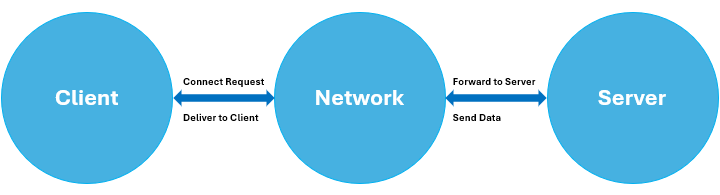
\includegraphics[width=1\textwidth]{2.png}
    \caption{System Organization Diagram}
    \label{fig:system_organization}
\end{figure}

\section{File Transfer Implementation}
\subsection{Client Code}
The following code snippet shows the implementation of the client in Python using TCP/IP for file transfer.

\begin{lstlisting}[language=Python, caption=Client Code for File Transfer]
#include <stdio.h>
#include <stdlib.h>
#include <unistd.h>
#include <string.h>
#include <arpa/inet.h>

#define SIZE 1024

void send_file(FILE *fp, int sockfd)
{
    char data[SIZE] = {0};

    while(fgets(data, SIZE, fp)!=NULL)
    {
        if(send(sockfd, data, sizeof(data), 0)== -1)
        {
            perror("Error in sendung data");
            exit(1);
        }
        bzero(data, SIZE);
    }
}

int main()
{
    char *ip = "127.0.0.1";
    int port = 8080;
    int e;

    int sockfd;
    struct sockaddr_in server_addr;
    FILE *fp;
    char *filename = "example.txt";
     sockfd = socket(AF_INET, SOCK_STREAM, 0);
    if(sockfd<0)
    {
        perror("Error in socket");
        exit(1);
    }
     printf("Server socket created. \n");

     server_addr.sin_family = AF_INET;
     server_addr.sin_port = port;
     server_addr.sin_addr.s_addr = inet_addr(ip);

     e = connect(sockfd, (struct sockaddr*)&server_addr, sizeof(server_addr));
     if(e == -1)
     {
         perror("Error in Connecting");
         exit(1);
     }
     printf("[+]Connected to server.\n");
     fp = fopen(filename, "r");
     if(fp == NULL)
     {
         perror("[-]Error in reading file.");
         exit(1);
     }
     send_file(fp,sockfd);
     printf("File data send successfully. \n");
     close(sockfd);
     printf("Disconnected from the server. \n");
     return 0;

}
\end{lstlisting}

\subsection{Server Code}
The following code snippet shows the server-side implementation to handle the incoming file and save it.

\begin{lstlisting}[language=Python, caption=Server Code for File Transfer]
#include <stdio.h>
#include <stdlib.h>
#include <string.h>
#include <arpa/inet.h>

#define SIZE 1024

void write_file(int sockfd)
{
    int n; 
    FILE *fp;
    char *filename = "received_file.txt";
    char buffer[SIZE];

    fp = fopen(filename, "w");
    if(fp==NULL)
    {
        perror("Error in creating file.");
        exit(1);
    }
    while(1)
    {
        n = recv(sockfd, buffer, SIZE, 0);
        if(n<=0)
        {
            break;
            return;
        }
        fprintf(fp, "%s", buffer);
        bzero(buffer, SIZE);
    }
    return;
    
}

int main ()
{
    char *ip = "127.0.0.1";
    int port = 8080;
    int e;

    int sockfd, new_sock;
    struct sockaddr_in server_addr, new_addr;
    socklen_t addr_size;
    char buffer[SIZE];

    sockfd = socket(AF_INET, SOCK_STREAM, 0);
    if(sockfd<0)
    {
        perror("Error in socket");
        exit(1);
    }
     printf("Server socket created. \n");

     server_addr.sin_family = AF_INET;
     server_addr.sin_port = port;
     server_addr.sin_addr.s_addr = inet_addr(ip);

     e = bind(sockfd,(struct sockaddr*)&server_addr, sizeof(server_addr));
     if(e<0)
     {
         perror("Error in Binding");
         exit(1);
     }
     printf("Binding Successfull.\n");

     e = listen(sockfd, 10);
     if(e==0)
     {
         printf("Listening...\n");
     }
     else 
     {
         perror("Error in Binding");
         exit(1);
     }
     addr_size = sizeof(new_addr);
     new_sock = accept(sockfd,(struct sockaddr*)&new_addr, &addr_size);

     write_file(new_sock);
     printf("Data written in the text file ");
}
\end{lstlisting}

\subsection{Implementing File Transfer}
\subsubsection{Testing with myself}
\begin{figure}[h]
    \centering
    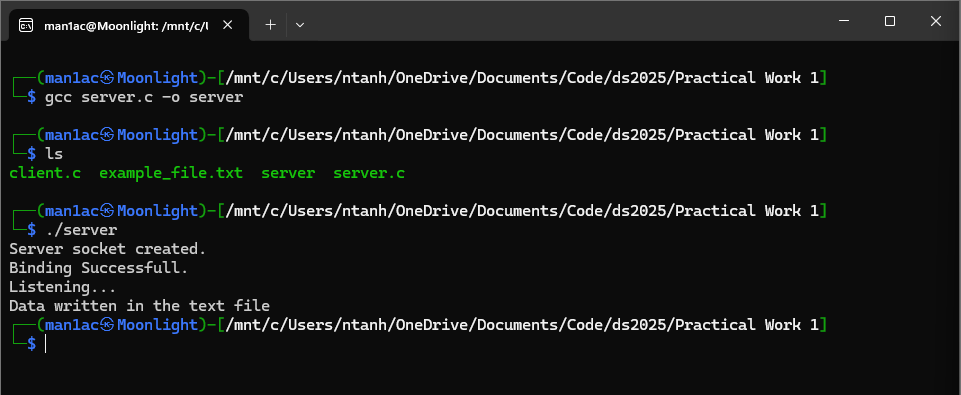
\includegraphics[width=1\textwidth]{3.png}
    \caption{Server Command Line Interface}
    \label{fig:server_command_line_interface}
\end{figure}

\begin{figure}[h]  
    \centering
    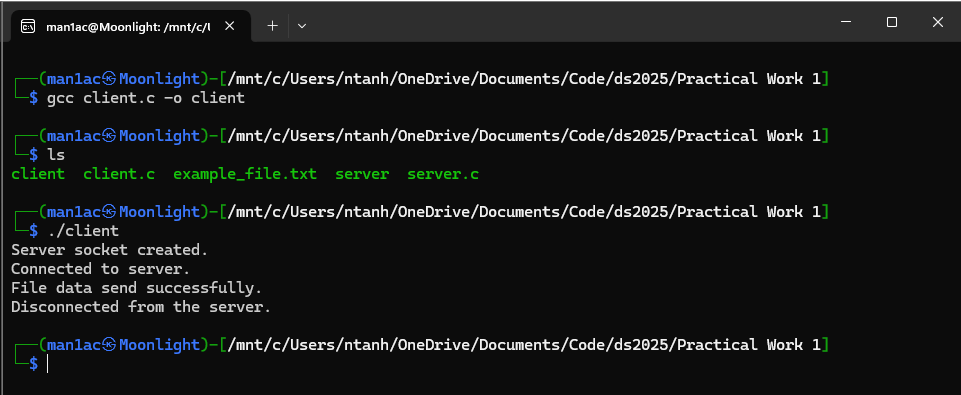
\includegraphics[width=1\textwidth]{4.png}
    \caption{Client Command Line Interface}
    \label{fig:client_command_line_interface}
\end{figure}

\section{Conclusion}
In this report, we have outlined the design and implementation of a file transfer system using TCP/IP in a Command Line Interface. The system allows for reliable file transfer between a client and a server. The custom protocol ensures efficient and secure transfer, and the implementation is robust enough to handle different file sizes.

\end{document}
